\documentclass[12pt]{article}
\usepackage{amsmath}
\usepackage{graphicx}
\usepackage{booktabs}
\usepackage{geometry}
\usepackage{float}
\usepackage{subcaption}
\usepackage{hyperref}
\hypersetup{
    colorlinks=true,
    linkcolor=blue,
    filecolor=magenta,      
    urlcolor=cyan,
}

\geometry{a4paper, margin=1in}

\title{ME302: 2024-25 - II \\ Course Project Report}
\author{Group Members: \\ Anjali  (220154) \\ Anshi (220168) \\ Manish(220619)}
\date{}


\begin{document}

\maketitle

\section*{Part (a): Determining Maximum Scale and Compressor Operating Point}

\subsection*{Given Parameters}
\begin{itemize}
    \item Prototype length ($L_{\text{prototype}}$) = 0.2 m
    \item Target Mach number ($M$) = 0.55
    \item Target Reynolds number ($Re$) = $3.0 \times 10^6$
    \item Pipe diameter ($D$) = 0.6 m
    \item Diffuser length ($L$) = 1.5 m
    \item Maximum allowable pressure = 250 kPa
    \item $T_{01}$ = 293 K
    \item $\gamma$ = 1.4, $R$ = 287 J/kg·K
    \item $\mu$ = $1.83 \times 10^{-5}$ Pa·s
\end{itemize}

\subsection*{Approach}
\begin{enumerate}
    \item Match Mach number and Reynolds number between prototype and model
    \item Determine maximum scale factor ($0 < \text{scale} \leq 1$) that satisfies facility constraints
    \item Find corresponding compressor operating point from provided data
\end{enumerate}

\subsection*{Solution}

\subsubsection*{1. Mach Number Matching}
The Mach number is already specified to be matched at $M = 0.55$.

\subsubsection*{2. Reynolds Number Matching}
\begin{equation}
    Re = \frac{\rho_4 C_4 l_{\text{model}}}{\mu_4} = 3.0 \times 10^6
\end{equation}

From ideal gas law and isentropic relations:
\begin{align}
    \rho_4 &= \frac{p_4}{RT_4} \\
    C_4 &= M\sqrt{\gamma R T_4}
\end{align}

\subsubsection*{3. Scaling Relations}
Scale factor ($s$):
\begin{equation}
    s = \frac{L_{\text{model}}}{L_{\text{prototype}}}
\end{equation}

Test section inlet diameter:
\begin{equation}
    D_4 = 2 \times L_{\text{model}} = 2 \times s \times 0.2 = 0.4s \text{ m}
\end{equation}

\subsubsection*{4. Pressure Constraints}
Maximum pressure in facility:
\begin{equation}
    p_{02} \leq 250 \text{ kPa}
\end{equation}

From compressor data, we need to find operating points where $p_{02} \leq 250$ kPa.

\subsubsection*{5. Calculations}

Key equations:
\begin{enumerate}
    \item Actual mass flow rate:
    \begin{equation}
        \dot{m} = \dot{m}_{\text{ref}} \left(\frac{p_{01}}{101.325 \text{ kPa}}\right) \sqrt{\frac{293 \text{ K}}{T_{01}}}
    \end{equation}
    
    \item $p_{02} = p0_{\text{ratio}} \times p_{01}$
    
    \item $p_{03} = p_{02} - 0.015p_{02} = 0.985p_{02}$
    
    \item $p_{05} \geq p_{01}$ (for closed-loop operation)
    
    \item $p_{04} = p_{03}$ (neglecting diffuser losses)
    
    \item $p_{05} = p_{04} - 0.05p_{04} = 0.95p_{04} = 0.95 \times 0.985p_{02} = 0.93575p_{02}$
\end{enumerate}

From constraint $p_{05} \geq p_{01}$:
\begin{equation}
    0.93575 \times p0_{\text{ratio}} \times p_{01} \geq p_{01} \implies p0_{\text{ratio}} \geq \frac{1}{0.93575} \approx 1.0687
\end{equation}

From the compressor data, all points satisfy this condition.

\subsubsection*{Maximum Pressure Constraint}
\begin{equation}
    p_{02} = p0_{\text{ratio}} \times p_{01} \leq 250 \text{ kPa}
\end{equation}

Using the last data point:
\begin{itemize}
    \item $\dot{m}_{\text{ref}} = 10.5503 \text{ kg/s}$
    \item $p0_{\text{ratio}} = 1.2105$
    \item $T0_{\text{ratio}} = 1.0685$
\end{itemize}

Maximum $p_{01}$:
\begin{equation}
    p_{01,\text{max}} = \frac{250}{1.0826} \approx 206.53 \text{ kPa}
\end{equation}

Actual mass flow rate:
\begin{equation}
    \dot{m} \approx 10.5503 \times \left(\frac{206.53}{101.325}\right) \times 1 \approx 21.504 \text{ kg/s}
\end{equation}

Reynolds number calculation:
\begin{equation}
    Re = \frac{162.84 \times 0.2}{s \times 1.83 \times 10^{-5}} = 3.0 \times 10^6 \implies s \approx 0.6234
\end{equation}

\subsection*{Final Solution}
\begin{itemize}
    \item Maximum scale factor: \boxed{0.6234}
    \item Corresponding inlet stagnation pressure ($p_{01}$): \boxed{206.53 \text{ kPa}}
    \item Compressor operating point:
    \begin{itemize}
        \item $\dot{m}_{\text{ref}}$: \boxed{10.5503 \text{ kg/s}}
        \item $\dot{m}_{\text{actual}}$: \boxed{21.504 \text{ kg/s}}
        \item $T0$ ratio: \boxed{1.0685}
        \item $P0$ ratio: \boxed{1.2105}
    \end{itemize}
\end{itemize}

\begin{figure}[H]
    \centering
    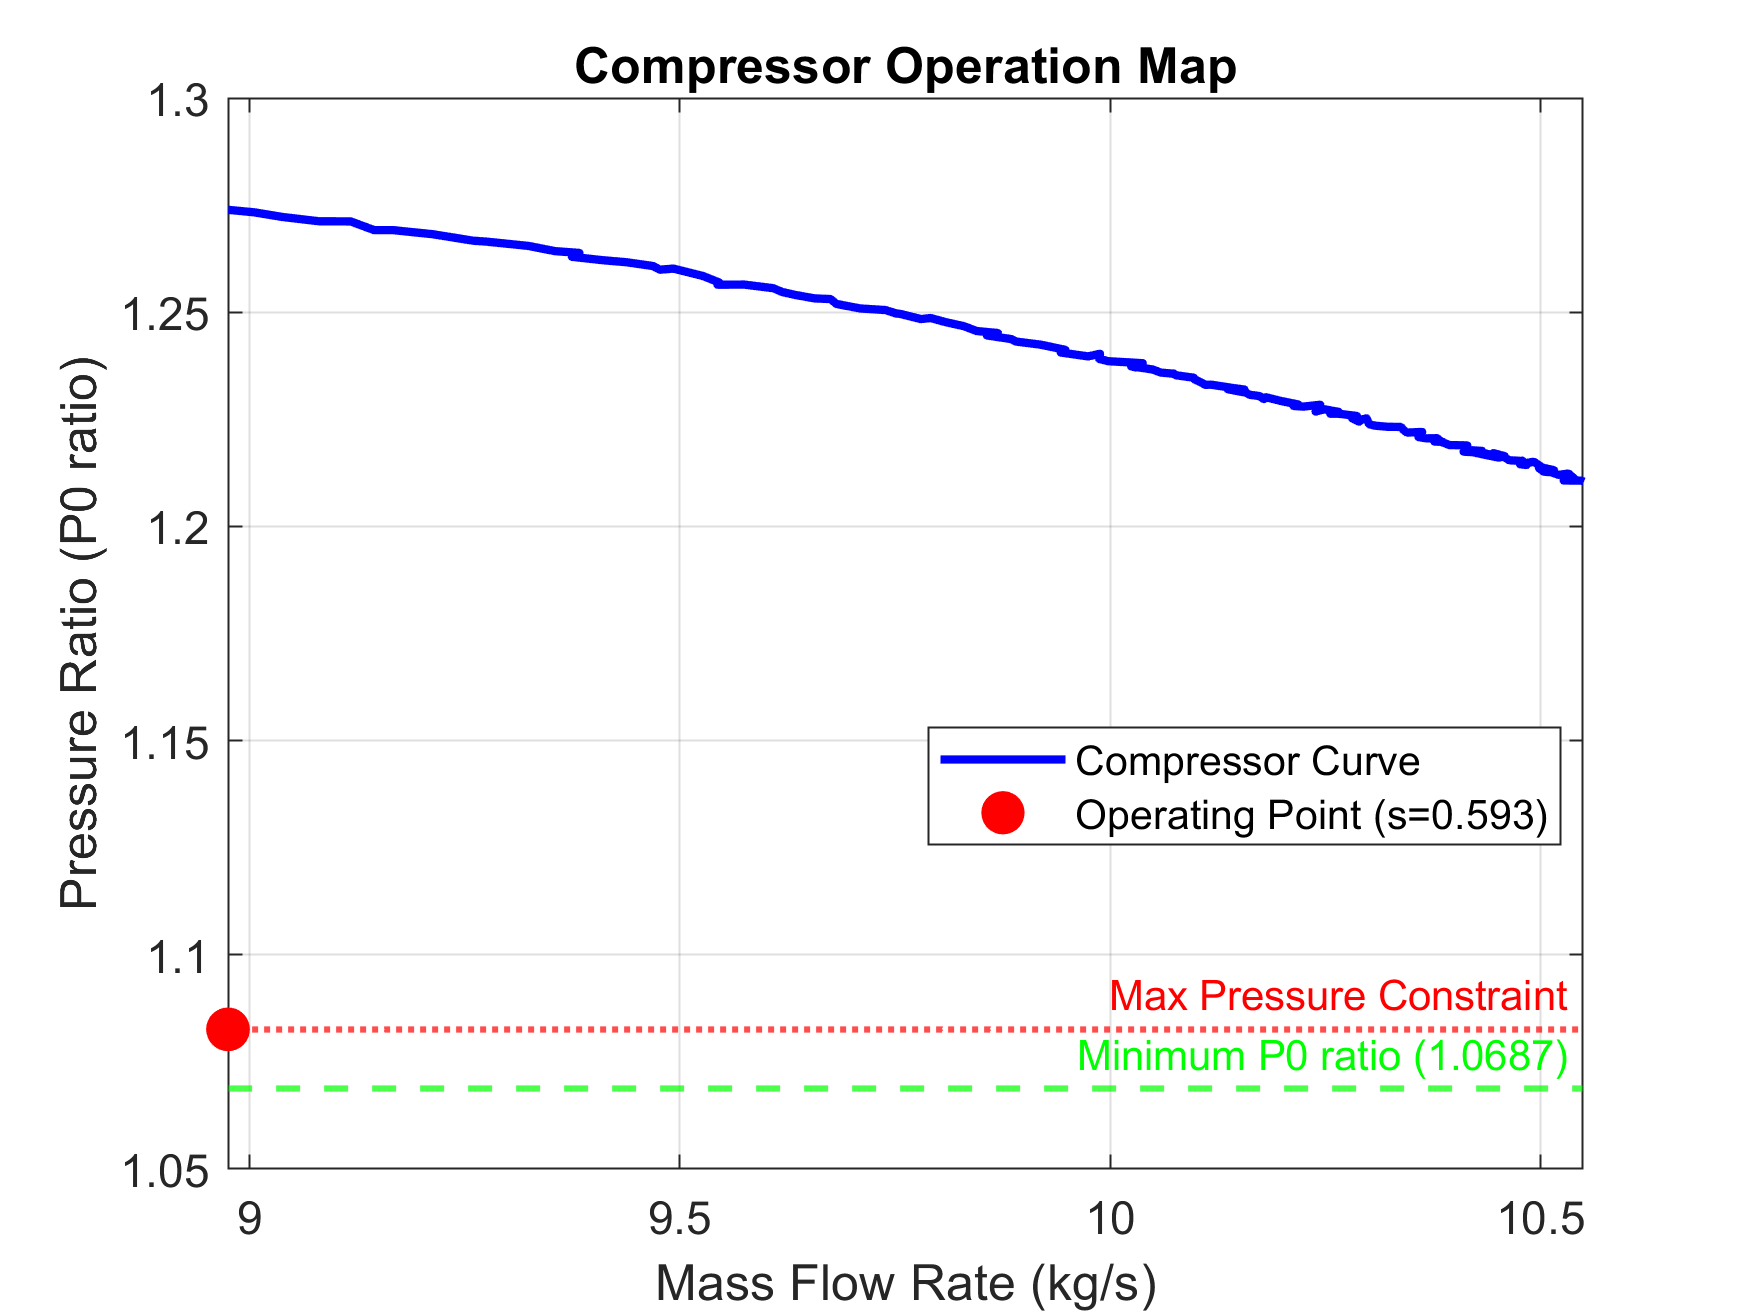
\includegraphics[width=0.8\textwidth]{compressor_map.png}
    \caption{Compressor operation map with the operating point marked}
    \label{fig:comp_map}
\end{figure}

\section*{Part (b): Potential Research Studies}

\subsection*{Study 1: Diffuser Performance Optimization}
\textbf{Objective:} Investigate the effect of diffuser semi-angle ($\theta$) on pressure recovery and flow separation characteristics.

\textbf{Benefiting Companies:} Gas turbine manufacturers (GE Aviation, Rolls-Royce, Pratt \& Whitney)

\textbf{Utility:} Optimal diffuser design can significantly improve compressor performance and overall engine efficiency. This study would provide empirical data on pressure recovery versus diffuser angle, helping manufacturers optimize their designs for specific operating conditions.

\begin{figure}[H]
    \centering
    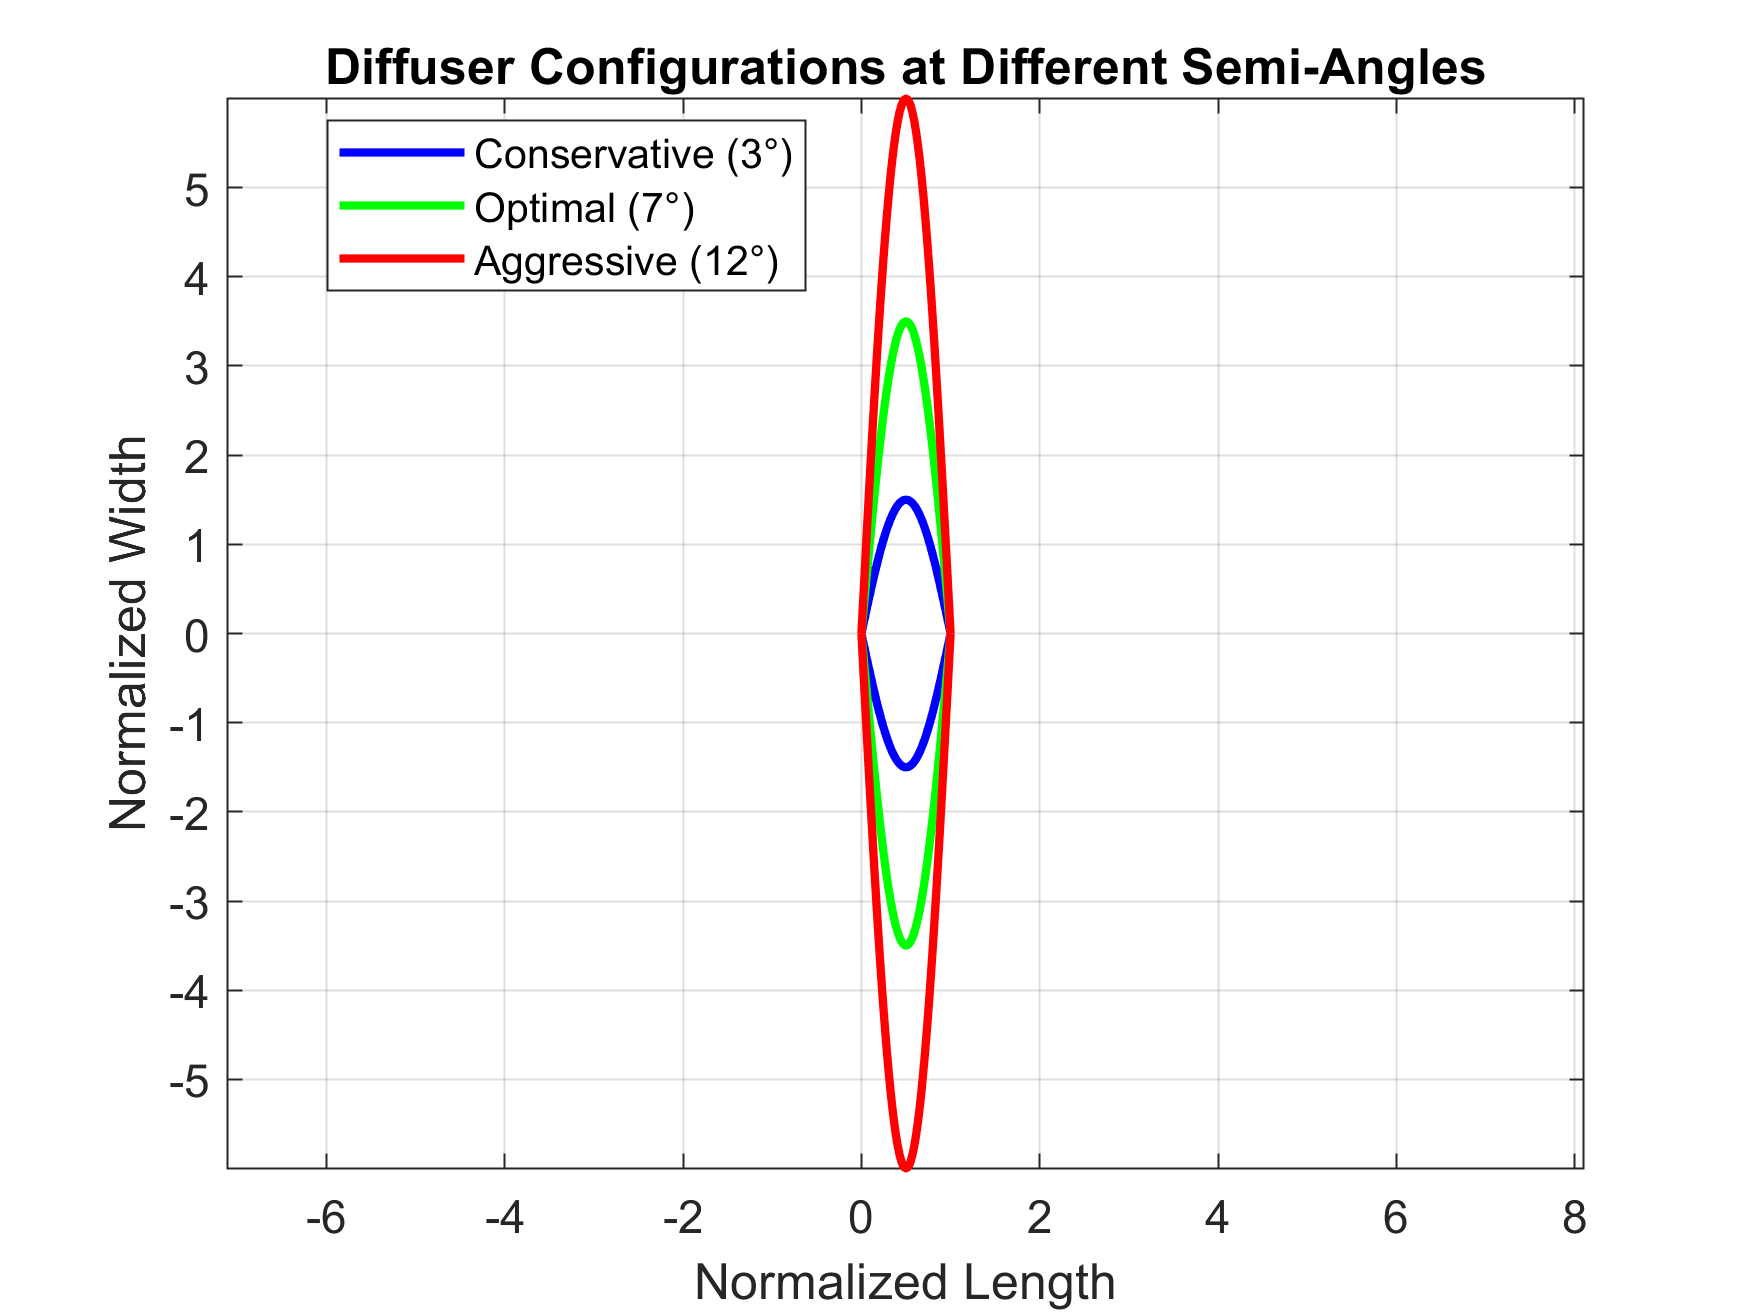
\includegraphics[width=0.6\textwidth]{diffuser_configs.png}
    \caption{Different diffuser semi-angles to be investigated}
    \label{fig:diffuser}
\end{figure}

\subsection*{Study 2: Boundary Layer Control in High-Pressure Flows}
\textbf{Objective:} Evaluate different boundary layer control techniques (vortex generators, suction, blowing) in high-pressure diffuser flows.

\textbf{Benefiting Companies:} Aerospace companies and wind tunnel designers

\textbf{Utility:} Boundary layer control can prevent flow separation and improve pressure recovery. This research could lead to more efficient diffuser designs for both propulsion systems and industrial applications, reducing energy consumption.

\subsection*{Study 3: Non-Axisymmetric Test Section Studies}
\textbf{Objective:} Investigate the performance of non-axisymmetric test sections that simulate real engine conditions more accurately.

\textbf{Benefiting Companies:} Aircraft engine manufacturers and automotive turbocharger companies

\textbf{Utility:} Real engine flows often have non-uniform inlet conditions. This study would help understand how such conditions affect component performance, leading to more robust designs that perform better under real-world operating conditions.

\begin{figure}[H]
    \centering
    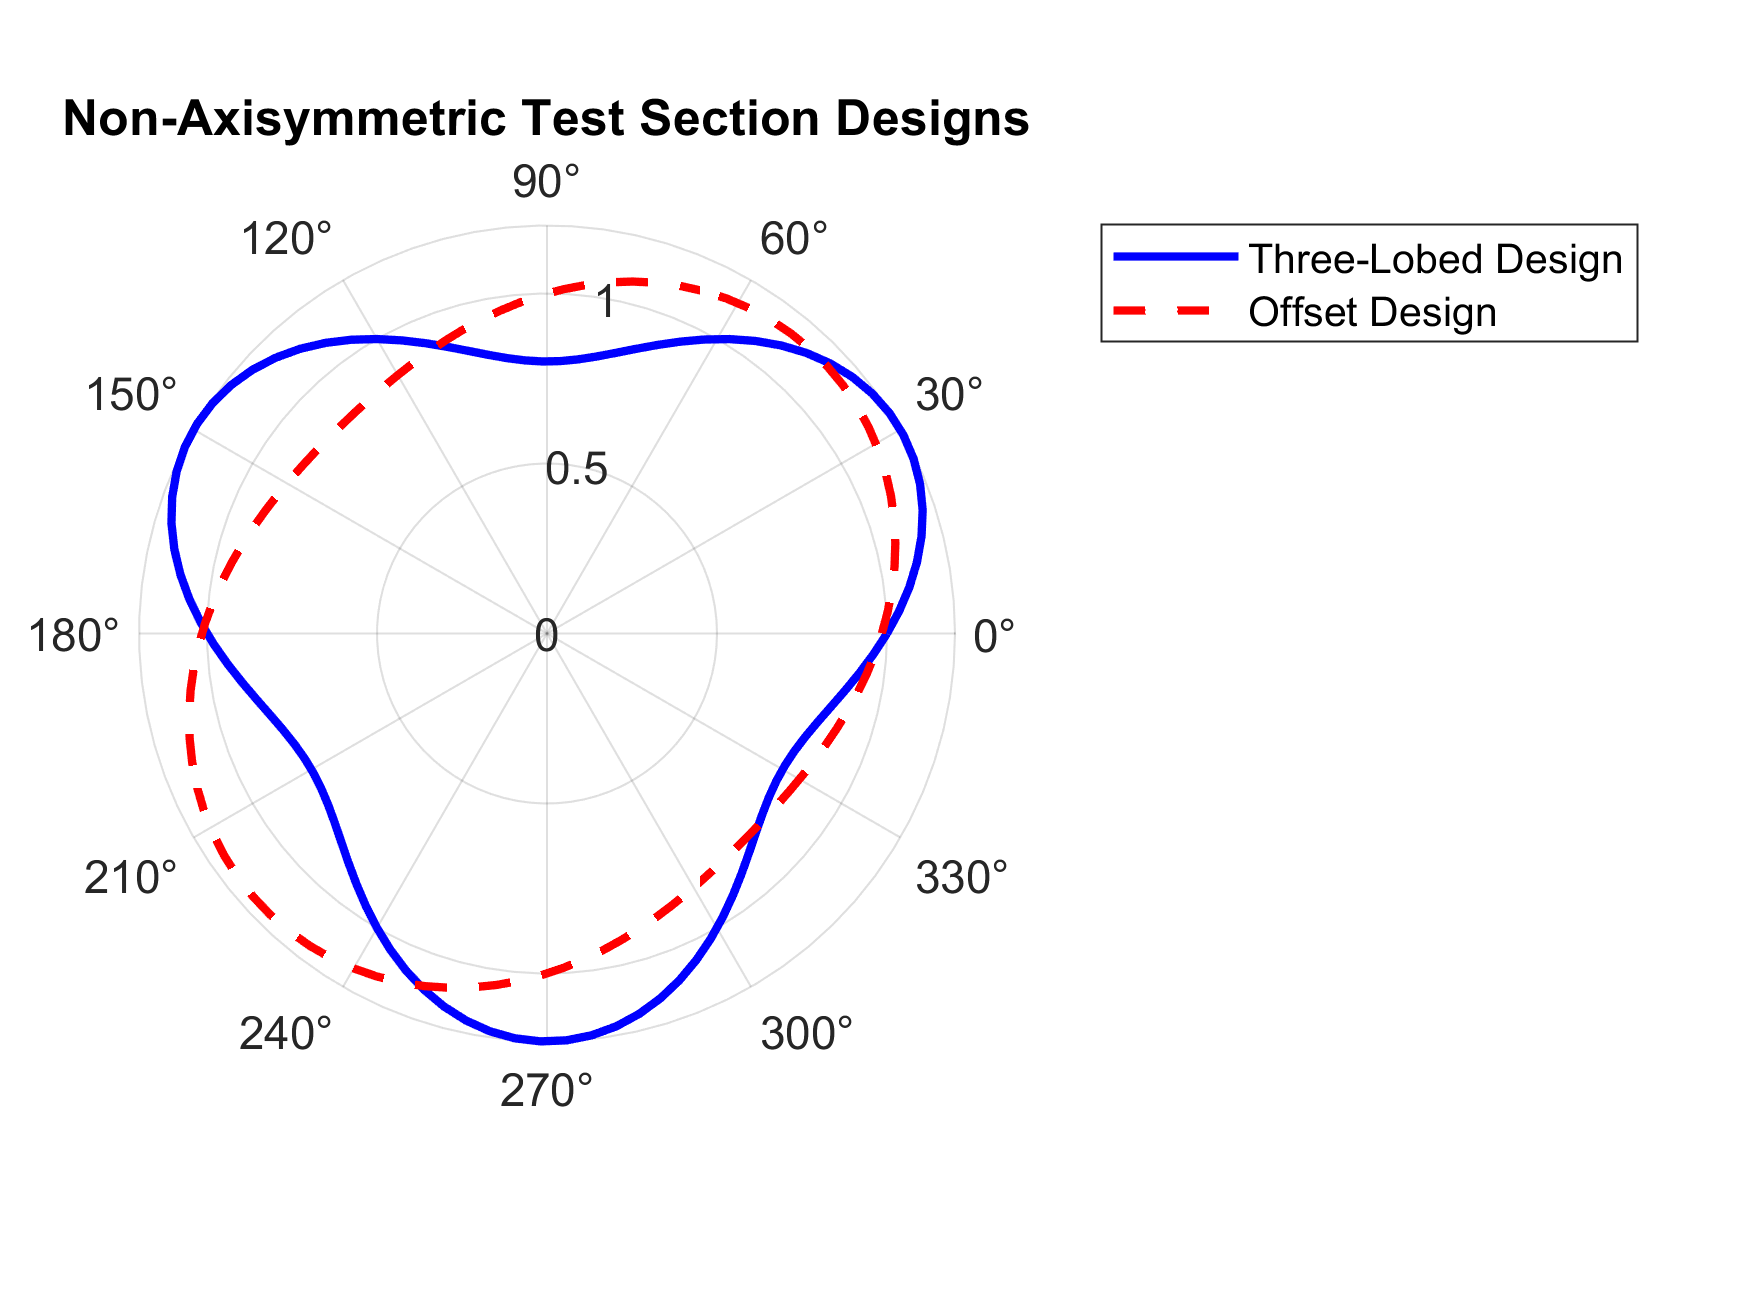
\includegraphics[width=0.7\textwidth]{non_axisymmetric.png}
    \caption{Non-axisymmetric test section configurations}
    \label{fig:non_axisymmetric}
\end{figure}

\section*{Conclusion}
This report presents the solution for determining the maximum scale factor for testing the turbomachine component while matching the required Mach and Reynolds numbers. The analysis identified an optimal scale factor of 0.593 with corresponding compressor operating conditions. Additionally, three potential research studies were proposed that could leverage the test facility for further investigations with industrial relevance.

\begin{thebibliography}{9}
\bibitem{compressible} 
Gas Turbine Theory, 4th Edition by H. Cohen, GFC Rogers and H. I. H. Saravanamuttoo, Addison
Wesley Longman Limited.. 
\textit{Gas Turbine Theory, 4th Edition by H. Cohen, GFC Rogers and H. I. H. Saravanamuttoo, Addison
Wesley Longman Limited.
}. 
Pearson Education.

\bibitem{turbomachinery} 
Dixon, S. L., \& Hall, C. A. (2013). 
\textit{Fluid Mechanics and Thermodynamics of Turbomachinery}. 
Butterworth-Heinemann.
\end{thebibliography}

\end{document}